\documentclass[12pt]{article}

\usepackage[margin=1in]{geometry} 
\usepackage{amsmath,amsthm,amssymb,mathtools}
\usepackage{graphicx}
\usepackage{tikz}
\usetikzlibrary{arrows}
\usepackage{pgfplots}
\pgfplotsset{compat=1.10}
\usepgfplotslibrary{fillbetween}
\usetikzlibrary{patterns}
\usepackage{setspace}
\onehalfspacing
\newcommand{\arrowIn}{
	\tikz \draw[-stealth] (-1pt,0) -- (1pt,0);
}
\date{}
\begin{document}
	\title{A solution method for Cournot oligopoly game with $2n$ players} \author{Chang Gao}
	\maketitle
	Consider a Cournot oligopoly game with 2$n$ players, allowing firms to face zero fixed cost and constant marginal cost. Single goods are produced. Half of the firms have type ‘$H$’ with unit product cost $c_H$ and the other half have type ‘$L$’ with unit product cost $c_L$. $c_L, c_H$ satisfies $0<c_L<c_H<1$.
	The demand function is given by
	\[ Q = \begin{cases} 
		1 - aP & 0 < P < \frac{1}{a} \\ 
		0 & P \geq \frac{1}{a}
	\end{cases}
	\]
	where $P$ is the price and $a>0$ is a constant. When the market clears, $Q$ is also the aggregate quantity produced by firms, therefore $Q\equiv\sum_{i=1}^{2n}q_i$.
	
	The cost to firm $i\in\{1,2,\cdots,2n\}$ of producing $q_i$ units of the good can be calculated
	
	\[ C_i(q_i) = \begin{cases} 
		c_L q_i & \text{if firm $i$ has type $L$} \\ 
		c_H q_i & \text{if firm $i$ has type $H$}
	\end{cases}
	\]
	
	Want to find the best reply of each firm and all (pure strategy) Nash equilibria. Explain the conditions for each type of equilibrium to exist.
	
	\medspace
	
	{\bf Cournot oligopoly game}
	\begin{itemize}
		\item Players: The 2$n$ firms
		\item Actions: Each firm’s set of actions is the set of its possible outputs
		\item Preference: Each firm’s preference is represented by its profit, $\pi_i(q_1,q_2,\cdots,q_{2n})=q_i P(q_1,q_2,\cdots,q_{2n})-C_i(q_i)$ for firm $i$.
	\end{itemize}
	
	\medspace
	\newpage
	
	{\bf 1. Solution for Cournot duopoly game ($2$ players case)}
	
	\medspace
	
	We can start solving this problem by analysing a duopoly game with two players.
	
	Suppose there are two firms producing the same good while their costs are different. A Nash equilibrium, in this case, is one pair $(q_L^*,q_H^*)$ of outputs for which $q_L^*$ is the best response to $q_H^*$, and $q_H^*$ is the best response to $q_L^*$.
	
	To find the Nash equilibrium, we can use a procedure based on the firms’ best response functions. To find firm L’s best response to any given output level of firm H, we need to study its profit as a function of its own output $q_L$. The profit function can be written $\pi_L(q_L;q_H)= P(q_L,q_H)q_L -C_L(q_L)$, where $q_H$ is the output of firm H, and we treat it as a given parameter here.
	
	%The inverse demand function is
	The profit function of firm H can be obtained in the same way, $\pi_H(q_H;q_L)= P(q_L,q_H)q_H -C_H(q_H)$. Therefore, we have
	
	\[ \pi_L(q_L;q_H) = \begin{cases} 
		-\frac{q_L^2}{a}+(\frac{1-q_H}{a}-c_L)q_L & q_H < 1-a c_L\\ 
		0 & q_H \geq 1-a c_L
	\end{cases}
	\]
	
	\medspace
	
	\[ \pi_H(q_H;q_L) = \begin{cases} 
		-\frac{q_H^2}{a}+(\frac{1-q_L}{a}-c_H)q_H & q_L < 1-a c_H\\ 
		0 & q_L \geq 1-a c_H
	\end{cases}
	\]
	
	\medspace
	
	Take the first order derivatives with respect to each firm's own production quantity. Let the first order condition equal to zero, $\frac{\partial(\pi_L(q_L;q_H))}{\partial q_L}=0$, $\frac{\partial(\pi_H(q_H;q_L))}{\partial q_H}=0$. Rearranging and obtain the best response functions
	
	\[ q_L(q_H) = \begin{cases} 
		-\frac{q_H}{2}+\frac{1-a c_L}{2} & q_H < 1-a c_L \\ 
		0 & q_H \geq 1-a c_L
	\end{cases}
	\]
	
	\medspace
	
	\[ q_H(q_L) = \begin{cases} 
		-\frac{q_L}{2}+\frac{1-a c_H}{2} & q_L < 1-a c_H \\ 
		0 & q_L \geq 1-a c_H
	\end{cases}
	\]
	
	\medspace
	
	Consider the fact $0<c_L<c_H<1$, we have $\frac{1-a c_H}{2}<\frac{1-a c_L}{2}<1-a c_L$ and $\frac{1-a c_H}{2}<1-a c_H<1-a c_L$. However, the relationship between $\frac{1-a c_L}{2}$ and $1-a c_H$ is unknown.
	
	Plugging positive part of firm L’s best response function into positive part of firm H’s, we obtain a possible interior solution $q_L^*=\frac{1-2a c_L+a c_H}{3}, q_H^*=\frac{1-2a c_H+a c_L}{3}$.
	
	Since $0<c_L<c_H<1$ and $a>0$ being a constant, $q_H$ is smaller than or equal to $q_L$ by nature. Therefore, the corner solution when $q_H>0$ and $q_L \leq 0$ does not exist. Both two firms will not produce a positive quantity for the same reason when $(q_ H < ) q_L \leq 0$.
	
	Then we can study the existing conditions for interior and corner solutions based on analysis of the best response function and the above solution.
	
	\medspace
	
	{\bf 1.1} Interior solution
	
	\medspace
	
	The following chart contains the two best response functions and helps show the incentives of firms for decision making when the best response functions intercept at positive quantities for both firms.
	
	\medspace
	
	\begin{center}
		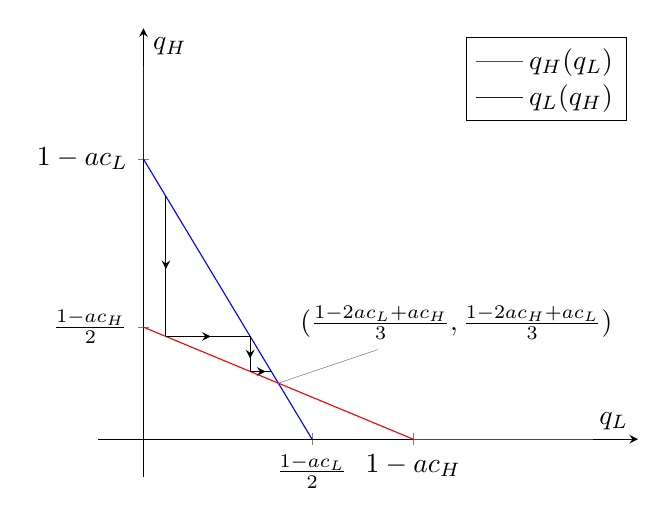
\begin{tikzpicture}
			\begin{axis}[axis lines=middle,
				xlabel=$q_L$,
				ylabel=$q_H$,
				enlargelimits,				
				xtick={1.5,2.4},
				ytick={1.2,3},
				xticklabels={$\frac{1-a c_L}{2}$,$1-a c_H$},
				yticklabels={$\frac{1-a c_H}{2}$,$1-a c_L$},],	
				\addplot[name path=b,red,domain={2.4:4}] {0};
				\addplot[name path=c,blue,domain={0:1.5}] {-2*x+3};
				\addplot[name path=a,red,domain={0:2.4}] {-0.5*x+1.2};
				\addplot[name path=d,blue,domain={-0.1:0.1}] coordinates {(0,3)(0,4)};
				\addplot[name path=e,white,domain={2.5:4}] {0.1};
				\node[coordinate,pin=70:{$(\frac{1-2a c_L+a c_H}{3},\frac{1-2a c_H+a c_L}{3})$}] at (axis cs:1.2,0.6){};
				\addplot[name path=f,black] coordinates {(0.2,2.6)(0.2,1.1)} node[
				sloped,
				pos=0.5,
				allow upside down]{\arrowIn};
				\addplot[name path=g,black] coordinates {(0.2,1.1)(0.95,1.1)}node[
				sloped,
				pos=0.5,
				allow upside down]{\arrowIn};
				\addplot[name path=h,black] coordinates {(0.95,1.1)(0.95,0.725)}node[
				sloped,
				pos=0.55,
				allow upside down]{\arrowIn};
				\addplot[name path=i,black] coordinates {(0.95,0.725)(1.1375,0.725)}node[
				sloped,
				pos=0.6,
				allow upside down]{\arrowIn};
				\addlegendentry{$q_H(q_L)$};
				\addlegendentry{$q_L(q_H)$};%first two plots
			\end{axis}
			
		\end{tikzpicture}
	\end{center}
	
	Now we can study the incentive of firms and find the solution. The best decisions for firms must be on the best response functions by their profit maximising motivations. Therefore, we can only pick the point on best response functions and make the analysis.
	
	We can pick an arbitrary state on the best response functions, say $a_1$. Firm H's best decision will lead to a new state $a_2$. However, it is not firm L's best response. Firm L's new response will bring the state $a_2$ to a new state $a_3$, and so on. Do the iteration repeatedly until it reaches a fixed point. Since the start point is arbitrary and the iteration always reaches the intercept in this linear case. This shows the interception of $q_H(q_L)$ and $q_L(q_H)$ is the unique solution for the duopoly game.
	
	The interior solution exists when the best response functions intercept at positive quantities for both firms, in other words, the interior solution exists when both $q_L^*$ and $q_H^*$ are greater than zero. These yield $\frac{1-2a c_L+a c_H}{3}>0$ and $\frac{1-2a c_H+a c_L}{3}>0$. Simplification yields $c_H<\frac{c_L}{2}+\frac{1}{2a}$. Market price in this equilibria is $\frac{1}{3a}+\frac{c_L}{3}+\frac{c_H}{3}$.
	
	\medspace
	
	{\bf 1.2} Corner solution
	
	\medspace
	
	The interior solution does not exist when the best response functions do not intercept at positive levels for both firms, which means at least one firm do not produce at a positive level. In this case, $\frac{1-a c_H}{2}<1-a c_H\leq\frac{1-a c_L}{2}<1-a c_L$, simplification\footnote{$c_H > 2 c_L-\frac{1}{a}$ could also be obtained here, this is satisfied by nature as $1-a c_L$ is always greater than $\frac{1-a c_H}{2}$.} yields $c_H\geq\frac{c_L}{2}+\frac{1}{2a}$.
	
	The following chart shows the best response functions in this case. The best response functions intercept at $(\frac{1-a c_L}{2},0)$ under such parameter conditions. 
	
	\medspace
	
	\begin{center}
		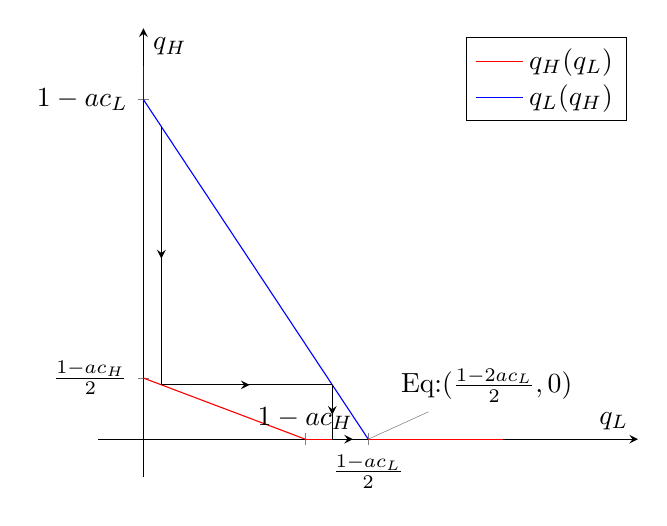
\begin{tikzpicture}
			\begin{axis}[axis lines=middle,
				xlabel=$q_L$,
				ylabel=$q_H$,
				enlargelimits,			
				xtick={1.8,2.5},
				ytick={0.9,5},
				xticklabels={,$\frac{1-a c_L}{2}$},
				yticklabels={$\frac{1-a c_H}{2}$,$1-a c_L$}],		
				\addplot[name path=a,red,domain={0:1.8}] {-0.5*x+0.9};
				\addplot[name path=c,blue,domain={0:2.5}] {-2*x+5};
				\addplot[name path=b,red,domain={1.8:4}] {0} node[black,pos=0, above]{$1-a c_H$};
				\addplot[name path=d,blue,domain={-0.1:0.1}] coordinates {(0,5)(0,5.5)};
				\addplot[name path=e,white,domain={2.5:5}] {0.1};
				\addplot[name path=f,black] coordinates {(0.2,4.6)(0.2,0.8)} node[
				sloped,
				pos=0.5,
				allow upside down]{\arrowIn};
				\addplot[name path=g,black] coordinates {(0.2,0.8)(2.1,0.8)}node[
				sloped,
				pos=0.5,
				allow upside down]{\arrowIn};
				\addplot[name path=h,black] coordinates {(2.1,0.8)(2.1,0)}node[
				sloped,
				pos=0.5,
				allow upside down]{\arrowIn};
				\addplot[name path=i,black] coordinates {(2.1,0)(2.5,0)}node[
				sloped,
				pos=0.5,
				allow upside down]{\arrowIn};
				\node[coordinate,pin=50:{Eq:$(\frac{1-2a c_L}{2},0)$}] at (axis cs:2.5,0){};
				\addlegendentry{$q_H(q_L)$};
				\addlegendentry{$q_L(q_H)$};%first two plots
			\end{axis}			
		\end{tikzpicture}
	\end{center}
	
	We can start to find the possible solution by using this chart. Like the interior solution case, pick an arbitrary state on the best response functions, say $a_1$. The iteration progress is the same until the last jump, in which case the state falls on somewhere between $1-a c_H$ and $\frac{1-a c_L}{2}$.
	
	The firm H will choose not to produce since the second last movement of firm L, $q_L$ before the last jump, is greater than or equal to $1-a c_H$. We can find the profit of firm H is 0 under such conditions by using the profit function we have listed before. If firm H choose a positive output in this case, its profit $\pi_H(q_H;q_L)=-\frac{q_H^2}{a}+(\frac{1-q_L}{a}-c_H)q_H$ is less than or equal to zero since $q_L \geq 1-a c_H$.
	
	Since $q_H$ is 0, the problem becomes firm L's profit maximising decision of choosing output level in $(1-a c_H,\frac{1-a c_L}{2})$ with $q_L$ being the total supply.
	
	The optimised output decision could be obtained by plugging $q_H=0$ into the best response function $q_L(q_H) = -\frac{q_H}{2}+\frac{1-a c_L}{2}$ where $q_H=0<1-a c_L$. So the corner solution is $(q_L^*,q_H^*)=(\frac{1-a c_L}{2},0)$, market price in this equilibria is $\frac{1}{2a}+\frac{c_L}{2}$.
	
	The above condition $\frac{1-a c_H}{2}<1-a c_H\leq\frac{1-a c_L}{2}<1-a c_L$ corresponds to $q_L(q_H)>0$ and $q_H(q_L) \leq 0$ in the sense of best response functions. We have known that $q_L>q_H$ is assured\footnote{In all solutions with different parameter conditions, $q_L\geq q_H$ is a necessary condition for the existence of the solution.}, and $q_L>q_H>0$ is the interior solution case. So, the corner solution where only firm L produces a positive output is the only possible outcome.
	
	\medspace
	
	
	{\bf 1.3} Other cases
	
	\medspace
	
	No solution other than $(0,0)$ exists in other cases since any positive output will lead to a negative profit for firms.
	
	\medspace
	
	{\bf Summary}
	
	\begin{itemize}
	
	\item The parameter condition for existence of interior solution is $c_H<\frac{c_L}{2}+\frac{1}{2a}$, where the equilibria is $(\frac{1-2a c_L+a c_H}{3},\frac{1-2a c_H+a c_L}{3})$ and the market price is $\frac{1}{3a}+\frac{c_L}{3}+\frac{c_H}{3}$. The market demand is $\frac{2-a c_L-a c_H}{3}$.
	
	\item The parameter condition for existence of corner solution is $c_H\geq\frac{c_L}{2}+\frac{1}{2a}$, where the equilibria is $(\frac{1-2a c_L}{2},0)$ and the market price is $\frac{1}{2a}+\frac{c_L}{2}$. The market demand is $\frac{1-a c_L}{2}$. The market price when firm H quits the market is lower since $\frac{1}{2a}+\frac{c_L}{2}-(\frac{1}{3a}+\frac{c_L}{3}+\frac{c_H}{3})=\frac{1}{6a}+\frac{c_L}{6}-\frac{c_H}{3}=\frac{1}{3}(\frac{c_L}{2}+\frac{1}{2a}-c_H)\leq 0$. The market demand when firm H quits the market is higher since $\frac{1-a c_L}{2}-\frac{2-a c_L-a c_H}{3}=\frac{(1-ac_L)-2(1-a c_H)}{6}>0$.
	
    \item When $(c_L,c_H)$ has other relationships, the solution is $(0,0)$.

    \end{itemize}
	
	We can use the chart\footnote{Both the white and blue shaded area can be the parameter conditions for the existence of corner solution.} below to describe the parameter conditions for existence of the solution.
	
	\medspace
	
	\begin{center}
		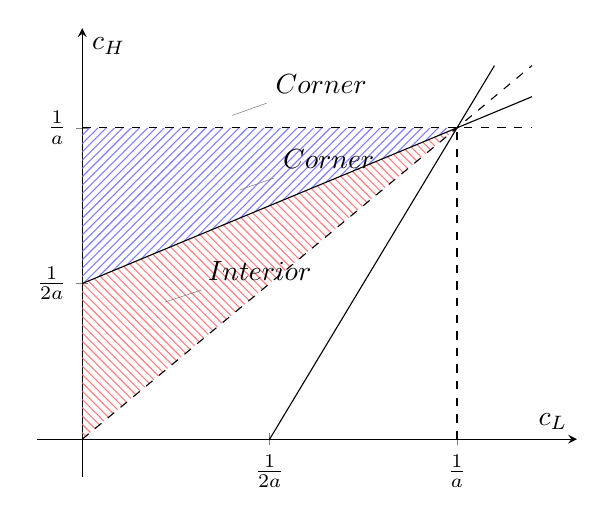
\begin{tikzpicture}
			\begin{axis}[axis lines=middle,
				xlabel=$c_L$,
				ylabel=$c_H$,
				enlargelimits,
				xtick={2.5,5},
				ytick={2.5,5},
				xticklabels={$\frac{1}{2a}$,$\frac{1}{a}$},
				yticklabels={$\frac{1}{2a}$,$\frac{1}{a}$}],		
				\addplot[name path=a,black,domain={2.5:5.5}] {2*x-5};
				\addplot[name path=b,black,domain={0:6}] {0.5*x+2.5};
				\addplot[name path=c,black,domain={0:6},dashed] {x};
				\addplot[name path=d,black,domain={0:6},dashed] {5};
				\addplot[name path=e,black,domain={0:6},dashed] coordinates {(5,0)(5,5)};
				\addplot[pattern=north west lines, pattern color=red!50]fill between[of=b and c, soft clip={domain=0:5}];
				\addplot[pattern=north east lines, pattern color=blue!50]fill between[of=b and d, soft clip={domain=0:5}];
				\node[coordinate,pin=20:{$Interior$}] at (axis cs:1.1,2.2){};
				\node[coordinate,pin=20:{$Corner$}] at (axis cs:2.1,4){};
				\node[coordinate,pin=20:{$Corner$}] at (axis cs:2,5.2){};
			\end{axis}
			
		\end{tikzpicture}
	\end{center}
	
	
	\noindent{\bf 2. Solution for Cournot oligopoly game with $2n$ players}
	
	\medspace
	
	Let us consider the game with 2$n$ players now.
	
	A Nash equilibrium (pure) here is one series $(q_1^*,q_2^*,\cdots,q_{2n}^*)$ of firms' outputs such that each $q_i^*$ is a best response to all other $q_j^*, j\neq i$. Assuming firm $i \in \{1,2,\cdots,n\}$ has low cost and firm $i \in \{n+1,n+2,\cdots,2n\}$ has high cost.
	
	The profit function for an individual firm is
	
	\[ \pi_i(q_i;q_1,q_2,\cdots,q_{i-1},q_{i+1},\cdots,q_{2n}) = \begin{cases} 
		q_i(\frac{1-\sum_{j=1}^{2n}q_j}{a}-c_L) & q_i < 1-a c_L - \sum_{j=1,j\neq i}^{2n}q_j\\ 
		0 & q_i \geq 1-a c_L - \sum_{j=1,j\neq i}^{2n}q_j
	\end{cases}
	\]
	
	for $i \in \{1,2,\cdots,n\}$, the low cost firms; and
	
	\[ \pi_i(q_i;q_1,q_2,\cdots,q_{i-1},q_{i+1},\cdots,q_{2n}) = \begin{cases} 
		q_i(\frac{1-\sum_{j=1}^{2n}q_j}{a}-c_H) & q_i < 1-a c_H - \sum_{j=1,j\neq i}^{2n}q_j\\ 
		0 & q_i \geq 1-a c_H - \sum_{j=1,j\neq i}^{2n}q_j
	\end{cases}
	\]
	
	for $i \in \{n+1,n+2,\cdots,2n\}$, the high cost firms.
	
	\medspace
	
	Take the first order derivatives of the above equation system with respect to each firm's own production quantity. Let the first order conditions equal to zero, $1-\sum_{j=1}^{2n} q_j-a c_i– q_i = 0$. (When $i \in \{1,2,\cdots,n\}$, let $c_i=c_L$; when $i \in \{n+1,n+2,\cdots,2n\}$, let $c_i=c_L$)
	
	Rearranging and get the best response functions
	
	\[ q_i(q_{\{j|j=1,2,\cdots,i-1,i+1,\cdots,2n\}}) = \begin{cases} 
		-\frac{\sum_{j=1,j \neq i}^{2n} q_j}{2}+\frac{1-a c_L}{2} & q_i < 1-a c_L - \sum_{j=1,j\neq i}^{2n}q_j \\ 
		0 & q_i \geq 1-a c_L - \sum_{j=1,j\neq i}^{2n}q_j
	\end{cases}
	\]
	
	for $i \in \{1,2,\cdots,n\}$, the low cost firms; and
	
	\[ q_i(q_{\{j|j=1,2,\cdots,i-1,i+1,\cdots,2n\}}) = \begin{cases} 
		-\frac{\sum_{j=1,j \neq i}^{2n} q_j}{2}+\frac{1-a c_H}{2} & q_i < 1-a c_H - \sum_{j=1,j\neq i}^{2n}q_j\\ 
		0 & q_i \geq 1-a c_H - \sum_{j=1,j\neq i}^{2n}q_j
	\end{cases}
	\]
	
	for $i \in \{n+1,n+2,\cdots,2n\}$, the high cost firms.
	
	\medspace
	
	Now we have got a linear equation system with $2n$ equations and $2n$ unknowns.
		
    \medspace
    
	{\bf 2.1} Interior solution
	
	\medspace
	
	Assume the interior solution exists, which means every firm produces at a positive level.
	
	In this case, we can sum up all the positive output parts of the best response functions. With $Q$ defined to be $\sum_{i=1}^{2n}q_i$, summations yields
	
	$$\sum_{i=1}^{2n}q_i=\frac{2n-(2nQ-Q)-na(c_L+c_H)}{2}(\equiv Q).$$
	
	This is an equation about $Q$, so we can solve for the total production and then solve for the price.
	
	$$Q=\frac{2n-na c_L-na c_H}{2n+1},$$
	
	$$P=\frac{1-Q}{a}=\frac{na(c_L+c_H)+1}{(2n+1)a}.$$
	
	In equilibria, the output for each firm is
	$q_i^*=\frac{na(c_H-c_L)+1-a c_L}{2n+1}$ for $i \in \{1,2,\cdots,n\}$;
	$q_i^*=\frac{na(c_L-c_H)+1-a c_H}{2n+1}$ for $i \in \{n+1,n+2,\cdots,2n\}$. This shows that the production quantity of low-cost firms is always higher than high-cost ones for the interior solution case. Surprisingly, best output level for firms with the same costs are the same.
	
	The necessary conditions in this case is $q_i < 1-a c_L - \sum_{j=1,j\neq i}^{2n}q_j$ for $i \in \{1,2,\cdots,n\}$ and $q_i < 1-a c_H - \sum_{j=1,j\neq i}^{2n}q_j$ for $i \in \{n+1,n+2,\cdots,2n\}$. This system could be simplified into $Q<1-a c_H<1-a c_L$. Since $Q=\frac{2n-na c_L-na c_H}{2n+1}$, we have $c_H<\frac{n a c_L+1}{(n+1)a}$.
	
	The existence and uniqueness of the interior solution could be proved by iteration. It could help show that the necessary condition above is sufficient for the existence of the interior solution.
	
	\medspace
	
	{\bf 2.2} Corner solution
	
	\medspace
	
	Since $0<c_L<c_H<1$ and $a>0$ being a constant, production quantity for low-cost firms is higher than that for high-cost firms by nature. It can be written $na(c_H-c_L)+1-a c_L >na(c_L-c_H)+1-a c_H$.
	
	The corner solution could only exist when some firms produce while some others do not produce. In other cases, no firm produces, or every firm produces, which is $(0,0)$ or an interior solution. So we need to study the incentives when some firms want to stay in the market while some others quit. Meanwhile, the output level for low-cost firms is always great than or equal to that of high-cost firms.
	
	So the only possible case is that at least some high-cost firms quit and some low-cost firms remain in the market. Using the best response functions, we have at least for some $(i,j)$ such that $q_i < 1-a c_L - \sum_{j=1,j\neq i}^{2n}q_j$ for $i \in \{1,2,\cdots,n\}$ and $q_j \geq 1-a c_H - \sum_{i=1,i\neq j}^{2n}q_i$ for $j \in \{n+1,n+2,\cdots,2n\}$. 
	
	This system could be simplified\footnote{$Q=q_j+\sum_{i=1,i\neq j}^{2n}q_i=q_i+\sum_{j=1,j\neq i}^{2n}q_j$} into $1-a c_H\leq Q<1-a c_L$.
	
	We can then find that, for firms with the same types, they are facing the same constraints by simply subtracting $q_i$ from $Q$ under the above inequality for $i\in{1,2,\cdots,2n}$.
	
	This implies that we sum up the firms who are producing at the positive output level; in other words, all the firms with low cost will produce a positive level. Only the $n$ low-cost firms produce under the above conditions. The best response functions are $q_i=-\frac{\sum_{j=1,j \neq i}^{n} q_j}{2}+\frac{1-a c_L}{2}$.
	
	Similarly, sum up the best response functions for remaining firms $Q^*=\frac{n-nQ^*+Q^*-nac_L}{2}$. Then we can calculate the demand and find the Nash equilibrium. In this case, in Nash equilibrium (pure), the best response for each remaining firm $i$ is $q_i^*=1-Q^*-a c_L=\frac{1-a c_L}{n+1}(\equiv\frac{Q^*}{n})$, the equilibrium price is $\frac{n a c_L +1}{(n+1)a}$. This can help us analyse the effect of increasing $n$ on consumer welfare in the following part. This also shows there exists a symmetric equilibrium where firms behave identically.
	
	\medspace
	
	{\bf 2.3} Other cases

	\medspace
	
	No solution other than $\{q_i^*=0|i=1,2,\cdots,2n\}$ exists in other cases since any positive output will lead to a negative profit for firms.
	
	\medspace
	
	{\bf Summary}
	
	\begin{itemize}
		
		\item The parameter condition for existence of interior solution is $c_H<\frac{na c_L+1}{(n+1)a}$, where the equilibria is $q_i^*=\frac{na(c_H-c_L)+1-a c_L}{2n+1}$ for low cost firms, $q_i^*=\frac{na(c_L-c_H)+1-a c_H}{2n+1}$ for high cost firms, the market price is $\frac{na(c_L+c_H)+1}{(2n+1)a}$ and the market demand is $\frac{2n-na c_L-na c_H}{2n+1}$.
		
		\item The parameter condition\footnote{$c_H>\frac{(n+1)ac_L-1}{na}$ is assured by the problem set up.} for existence of corner solution is $c_H\geq\frac{na c_L+1}{(n+1)a}$, where the equilibria is produce $\frac{1-a c_L}{n+1}$ for each remaining low-cost firm and the market price is $\frac{1+na c_L}{(n+1)a}$. The market demand is $\frac{n(1-a c_L)}{n+1}$. The market price when firms with high cost quit the market is lower since $\frac{1+na c_L}{(n+1)a}-\frac{na(c_L+c_H)+1}{(2n+1)a}=\frac{n^2 a c_L+n}{(n+1)(2n+1)a}-\frac{n c_H}{2n+1}=\frac{n}{2n+1}(\frac{n a c_L+1}{(n+1)a}-c_H)\leq 0$. The market price when firms with high cost quit the market is higher since $\frac{n(1-a c_L)}{n+1}-\frac{2n-na c_L-na c_H}{2n+1}=\frac{n[n(1-a c_L)-(n+1)(1-a c_H)]}{(n+1)(2n+1)}>0$.
		
		
		
		\item When $(c_L,c_H)$ has other relationships, the solution is $\{q_i^*=0|i=1,2,\cdots,2n\}$.
		
	\end{itemize}

We can use the chart\footnote{Both the white and blue shaded area can be the parameter conditions for the existence of corner solution.} below to describe the parameter conditions for the existence of solutions.

\medspace

\begin{center}
	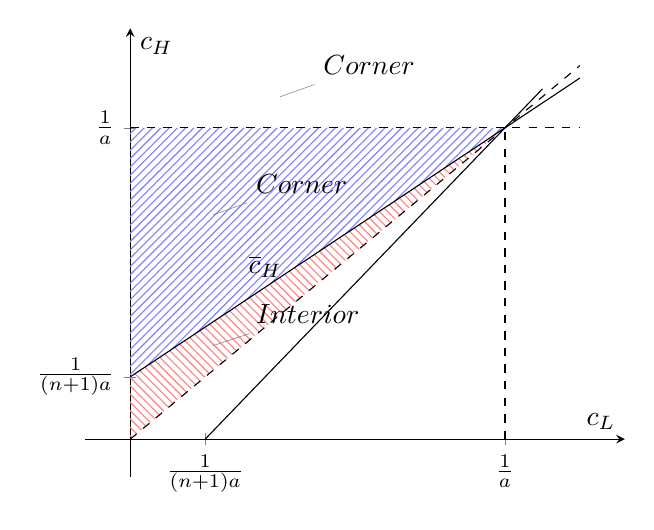
\begin{tikzpicture}
		\begin{axis}[axis lines=middle,
			xlabel=$c_L$,
			ylabel=$c_H$,
			enlargelimits,
			xtick={1,5},
			ytick={1,5},
			xticklabels={$\frac{1}{(n+1)a}$,$\frac{1}{a}$},
			yticklabels={$\frac{1}{(n+1)a}$,$\frac{1}{a}$}],		
			\addplot[name path=a,black,domain={1:5.5}] {1.25*x-1.25};
			\addplot[name path=b,black,domain={0:6}] {0.8*x+1}node[pos=.3, above]{$\overline c_H$};
			\addplot[name path=c,black,domain={0:6},dashed] {x};
			\addplot[name path=d,black,domain={0:6},dashed] {5};
			\addplot[name path=e,black,domain={0:6},dashed] coordinates {(5,0)(5,5)};
			\addplot[pattern=north west lines, pattern color=red!50]fill between[of=b and c, soft clip={domain=0:5}];
			\addplot[pattern=north east lines, pattern color=blue!50]fill between[of=b and d, soft clip={domain=0:5}];
			\node[coordinate,pin=20:{$Interior$}] at (axis cs:1.1,1.5){};
			\node[coordinate,pin=20:{$Corner$}] at (axis cs:1.1,3.6){};
			\node[coordinate,pin=20:{$Corner$}] at (axis cs:2,5.5){};
		\end{axis}
	\end{tikzpicture}
\end{center}
	
	\medspace
	
	\noindent{\bf 3. Changes in welfare according to changes in $n$}
	
	\medspace
	
	We can use a cutoff $\overline c_H\coloneqq \frac{na c_L+1}{(n+1)a}$ to help understand the comparative statics. $\frac{\partial \overline c_H}{\partial n}=\frac{a(a c_L-1)}{(n+1)^2a^2}<0$, which shows a downward shifting trend\footnote{The partial derivative is always less than zero because $a c_L$ has to be less than one. Otherwise, the output could be non-positive. For example, when $n=1$, $1- a c_L$ have to be positive. Thus a necessary condition for the existence of the interior solution.} of the cutoff condition $c_H$ when $n$ becomes larger.
	
	The intercept of the cutoff line $\overline c_H$ on $c_H$, $\frac{1}{(n+1)a}$ on $c_H$ in the second graph converges to 0 as $n\rightarrow\infty$. The cutoff line itself is also getting closer to $c_H=c_L$ as $n$ becomes larger. This implies when more firms compete, the condition for high-cost firms to remain involved is becoming stricter.
	
	We can compare the equilibrium price for the interior solution and corner solution.
	
	$$P_{interior}=\frac{na(c_L+c_H)+1}{(2n+1)a},$$
	
	$$P_{corner}=\frac{na c_L+1}{(n+1)a}.$$
	
	When $n\rightarrow\infty$, $P_{interior}\rightarrow\frac{c_L+c_H}{2}$ is greater than $P_{corner}\rightarrow c_L$ since $c_H>c_L$. This shows the improvement of efficiency brought by more competitors. The intuitions is that more competitors make the high-cost firms have less market share, whose profit converges to 0 as $\overline c_H$ get closer to $c_H=c_L$. The difference between $\frac{c_L+c_H}{2}$ and $c_L$ prompts the high-cost firms to exit the market.
	
\end{document}